\documentclass[12pt, letterpaper, titlepage]{article}

\usepackage{amsmath, amsfonts}
\usepackage{booktabs}
\usepackage{amsthm}
\usepackage{graphicx}
\usepackage[margin=1in]{geometry}
\usepackage{hyperref}
\usepackage{cleveref}
\hypersetup{colorlinks = true, linkcolor = blue, citecolor=blue, urlcolor = blue}
\usepackage{natbib}
\usepackage{float}
\usepackage{setspace}
\usepackage{pdfpages}
\usepackage[pagewise]{lineno}
\usepackage{mwe}
\usepackage{comment}
%\linenumbers*[1]
% %% patches to make lineno work better with amsmath
\newcommand*\patchAmsMathEnvironmentForLineno[1]{%
 \expandafter\let\csname old#1\expandafter\endcsname\csname #1\endcsname
 \expandafter\let\csname oldend#1\expandafter\endcsname\csname end#1\endcsname
 \renewenvironment{#1}%
 {\linenomath\csname old#1\endcsname}%
 {\csname oldend#1\endcsname\endlinenomath}}%
\newcommand*\patchBothAmsMathEnvironmentsForLineno[1]{%
 \patchAmsMathEnvironmentForLineno{#1}%
 \patchAmsMathEnvironmentForLineno{#1*}}%

\AtBeginDocument{%
 \patchBothAmsMathEnvironmentsForLineno{equation}%
 \patchBothAmsMathEnvironmentsForLineno{align}%
 \patchBothAmsMathEnvironmentsForLineno{flalign}%
 \patchBothAmsMathEnvironmentsForLineno{alignat}%
 \patchBothAmsMathEnvironmentsForLineno{gather}%
 \patchBothAmsMathEnvironmentsForLineno{multline}%
}

% control floats
\renewcommand\floatpagefraction{.9}
\renewcommand\topfraction{.9}
\renewcommand\bottomfraction{.9}
\renewcommand\textfraction{.1}
\setcounter{totalnumber}{50}
\setcounter{topnumber}{50}
\setcounter{bottomnumber}{50}

\newcommand{\jy}[1]{\textcolor{blue}{JY: #1}}
\newcommand{\eds}[1]{\textcolor{red}{EDS: (#1)}}
\newcommand{\of}[1]{\textcolor{violet}{OF: #1}}


\title{STAT 5225 Final Project} 

\author{Owen Fiore\\
%   \href{mailto:owen.fiore@uconn.edu}
% {\nolinkurl{owen.fiore@uconn.edu}}\\
}
\date{}

\begin{document}
\maketitle


\begin{abstract}
Looking at data from 2012 to 2021 of drug overdoses in Connecticut, an analysis was performed to try and determine any trends in the data and see if there were any correlations between features and drug overdose deaths. It was found that there has been a substantial increase in drug related deaths from 2012 to 2021 in Connecticut, and that there are trends for sex, race, and income in the data.

\end{abstract}

\doublespace

%The injury column may be bc this was subsetted from a larger data set that included people who died
%include summary of missing data

\section{Introduction} \label{sec:intro}
The dataset comes from the state of Connecticut and the base data contains 48 columns and 9,202 rows with each row representing a death \citep{data}.  Columns contain information about where the overdose happen, general information about the person (sex, age, residence, etc.), and information about the drug(s) found in the deceased's system.  It is important to understand that not all columns in the data are predictors, as some contain information about the types of drugs found in the deceased.

The contribution of this paper is to analyze the Accidental Drug Related Deaths 2012-2021 database to try to gain a deeper understanding of what factors can impact drug overdoses.  This is a very important topic, because in recent years, the opioid crisis has finally been covered by the mainstream media.  The leading cause of accidental deaths in Connecticut every year from 1999 to 2013 was drugs and in 2013 the number of drug related deaths was nearly double that of motor vehicle accidents \citep{tran_2022}.  Tran's study also found that in 2013 and 2014 Connecticut was above the United States average in drug and opioid overdose deaths (His data/analysis ended in 2014).  An investigation into the data to try and find any trends in order to understand what factors impact drug overdose deaths.


\section{Data} \label{sec:Data}
There are eighteen different drugs that serve as features and the data is coded as ``Y" if that specific drug was found in an autopsy/blood toxicology report of the deceased and left blank otherwise.  In many cases, multiple drugs were found in the body of the deceased, meaning that is difficult to know the true cause of death.  We can augment the data by finding additional data that can help better describe the columns of the data.  For example, knowing the city that the deceased lived or died in; is very difficult to interpret.  Towns such as ``Fairfield", ``New Haven", ``Hebron" are all different and are composed of different demographics.  That is why a database containing information such as per capita income can be helpful in trying to understand who it was that died.  There is no way to know the economic status of someone who died, but this gives us some context as to what kind of town that they lived in.


\section{Methods} \label{sec:Methods}
This paper attempted to utilize unsupervised learning techniques to learn about the data through using hierarchical clustering in R.  However, there were major issues with implementing the ``NbClust" package in R such as the runtime being too long and the height of the dendrogram depicting the hierarchical clustering not being interpretable.  Principal component analysis was also considered to reduce the dimensionality of the dataset, but this too was abandoned due to interpretability concerns.  One of the more difficult parts of this dataset was that this simply shows everyone that died, but does not contain any information about anyone who used drugs and lived, that is why it is difficult to do any modeling of the data.  That would require feature labels on whether somebody died, and then classification methods could be implemented to find factors that are heavily correlated with death.  Thus, as a result histograms were used to count the number of occurrences in the data, with the belief that high occurrences may indicate a correlation between drug overdoses.  We can also compare demographics to known demographics in the state of Connecticut to see if the deceased are representative of Connecticut's population as a whole.




\section{Results} \label{sec:Results}

\begin{figure}[tbp]
    \centering
    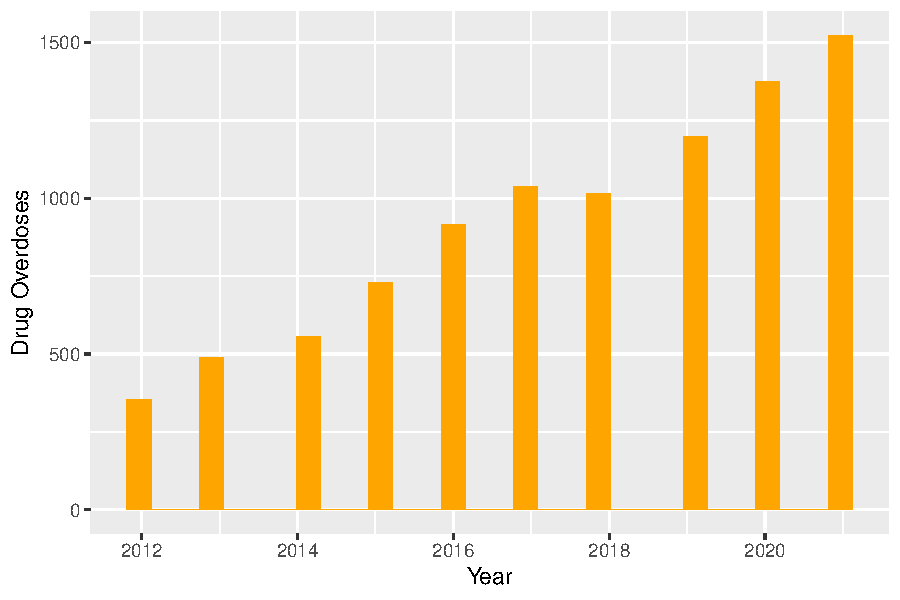
\includegraphics{OD_per_year}
    \caption{Drug Overdoses per year from 2012 to 2021 in CT.}
    \label{fig:OD_per_year}
  \end{figure}

Graph~\ref{fig:OD_per_year} shows the number of drug overdoses each year from 2012 to 2021 in Connecticut.  Note that there is a strong upward trend in the data, indicating that the opioid crisis is becoming a larger issue.  There were over three times as many overdoses in 2021 compared to 2023.  The only drop in deaths occurred from 2017 to 2018, and the decrease was minimal.

\begin{figure}[tbp]
    \centering
    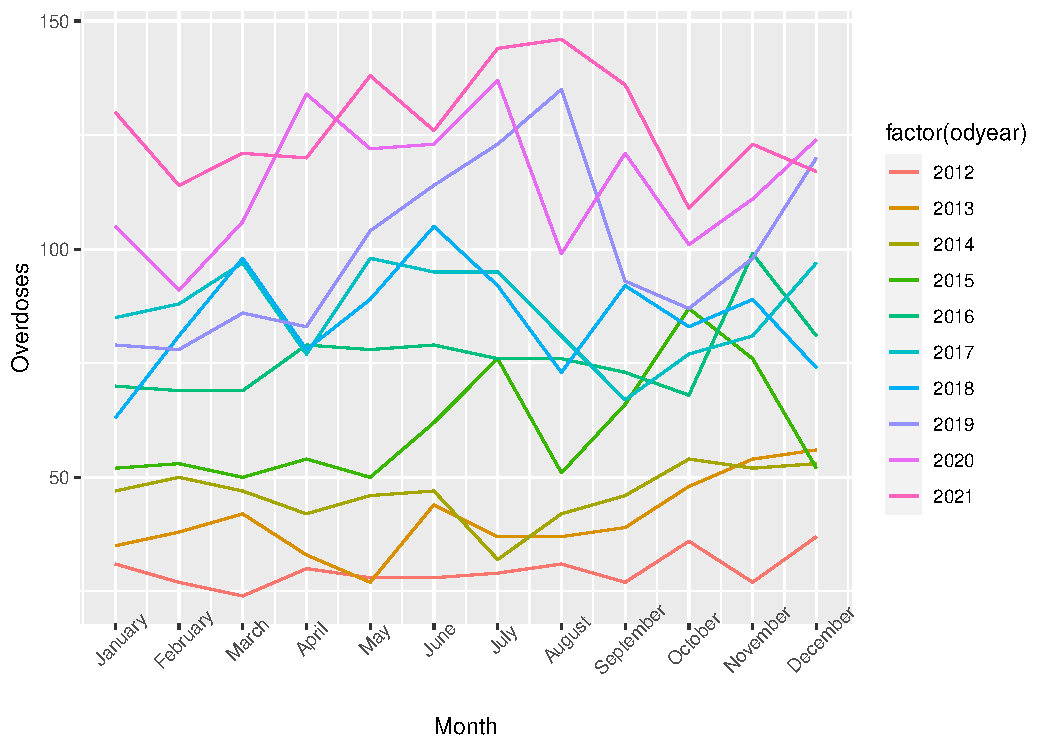
\includegraphics{Colorline}
    \caption{Drug Overdoses by month from 2012 to 2021 in CT.}
    \label{fig:Colorline}
  \end{figure}

Graph~\ref{fig:Colorline} shows each year's monthly drug overdose deaths to show how even with some noise each month, generally each year has more deaths than the year before.  There seems to be a slight trend of drug overdoses rising during the warm months: May-August and that deaths tend to taper off in November-January.
Another thing that is important about Graph~\ref{fig:Colorline} is that it shows that the distribution of deaths over the span of the year is different for every month.  2012 had the most consistent line, with there being roughly 30 to 40 deaths each month.  2019 by contrast had anywhere from 80 to 135 deaths each month. 

\begin{figure}[tbp]
    \centering
    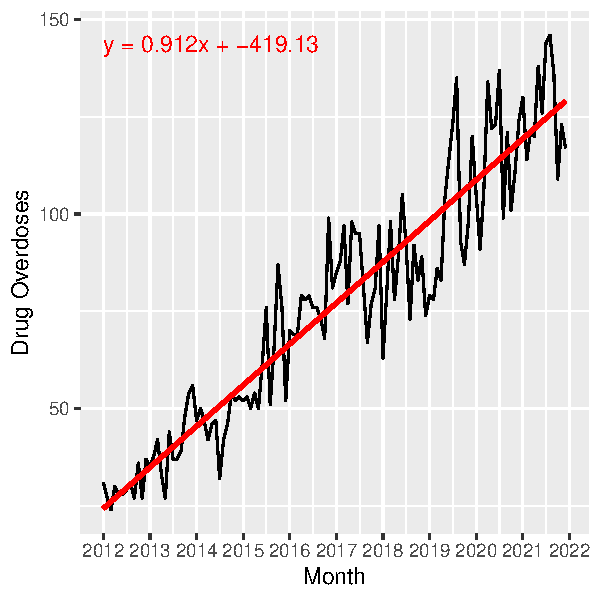
\includegraphics{Trendline}
    \caption{Drug Overdoses by month from 2012 to 2021 in CT.}
    \label{fig:Trendline}
  \end{figure}

While Graph~\ref{fig:OD_per_year} looked at the number of overdoses per year, but we can also look at the number of overdoses by month.  Graph~\ref{fig:Trendline} is a line graph that shows the number of overdoses by month.  Also included is the linear model fit parameters: slope and intercept to show that the number of overdoses per month is increasing.  The slope of the linear fit is 0.912, which indicates that for every month from January 2012 to December 2021, the number of people dying from drug overdoses each month increased on average by 0.912.  Over the 108 month span, the number of deaths increased on average from roughly 25 at the start of 2012 to over 125 by the end of 2021.

It is also important that we try to find factors in the data that we think can have an effect on death.  Although it has been established that we cannot perform any methods that require labels and prediction, but we can use histograms to show the counts to see how frequent certain values appear in the data.  We can start this off by finding the most common ages that appeared in the data.  Histogram~\ref{fig:AgeHist} shows that it is primarily young adults and middle-aged people that are dying of drug overdoses in Connecticut.  The histogram appears to be bimodal which is interesting: the data peaks for 35-36 year olds but then reaches a local minimum for 41-42 year olds before climbing and peaking again for 49-50 year olds.  After this there is a taper off all the way down to about 75.  Something that is slightly surprising is how old some people dying of drug overdoses in Connecticut.  There has long been a stigma that it is the youth who are using drugs such as heroin, fentanyl, etc. but there are clearly older users of prescription drugs too.

\begin{figure}[tbp]
    \centering
    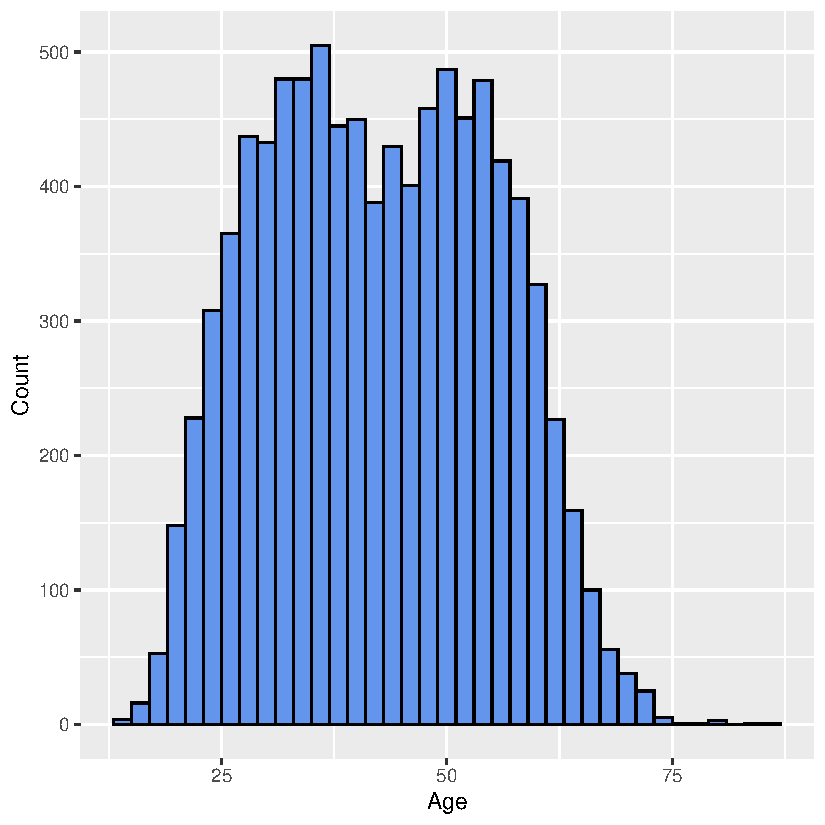
\includegraphics{MoneyHistogram}
    \caption{Distribution of ages over the data. Note that each bar represents two years.}
    \label{fig:AgeHist}
  \end{figure}

Besides age, two other important factors are gender and race.  Figure~\ref{fig:SexHist} shows that males make up a large share of the data, with almost 75\% of the drug overdose deaths being men.  Figure~\ref{fig:RaceHist} shows the distribution of overdoses by race.  A vast majority of the deaths from 2012-2021 were white, with Blacks and African Americans making up a significant amount of the rest of the non-white population. Section~\ref{sec:Discussion} provides context as to why so many of the deceased were white.

\begin{figure}[tbp]
    \centering
    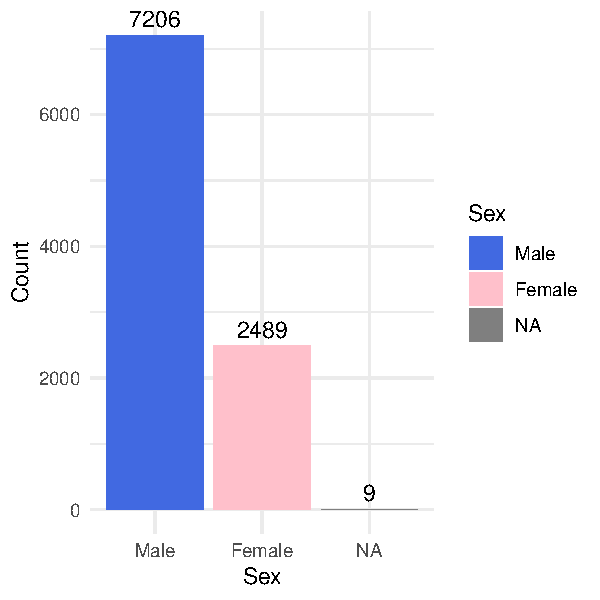
\includegraphics{SexHist}
    \caption{Counts of drug overdoses by sex.}
    \label{fig:SexHist}
  \end{figure}

  \begin{figure}[tbp]
    \centering
    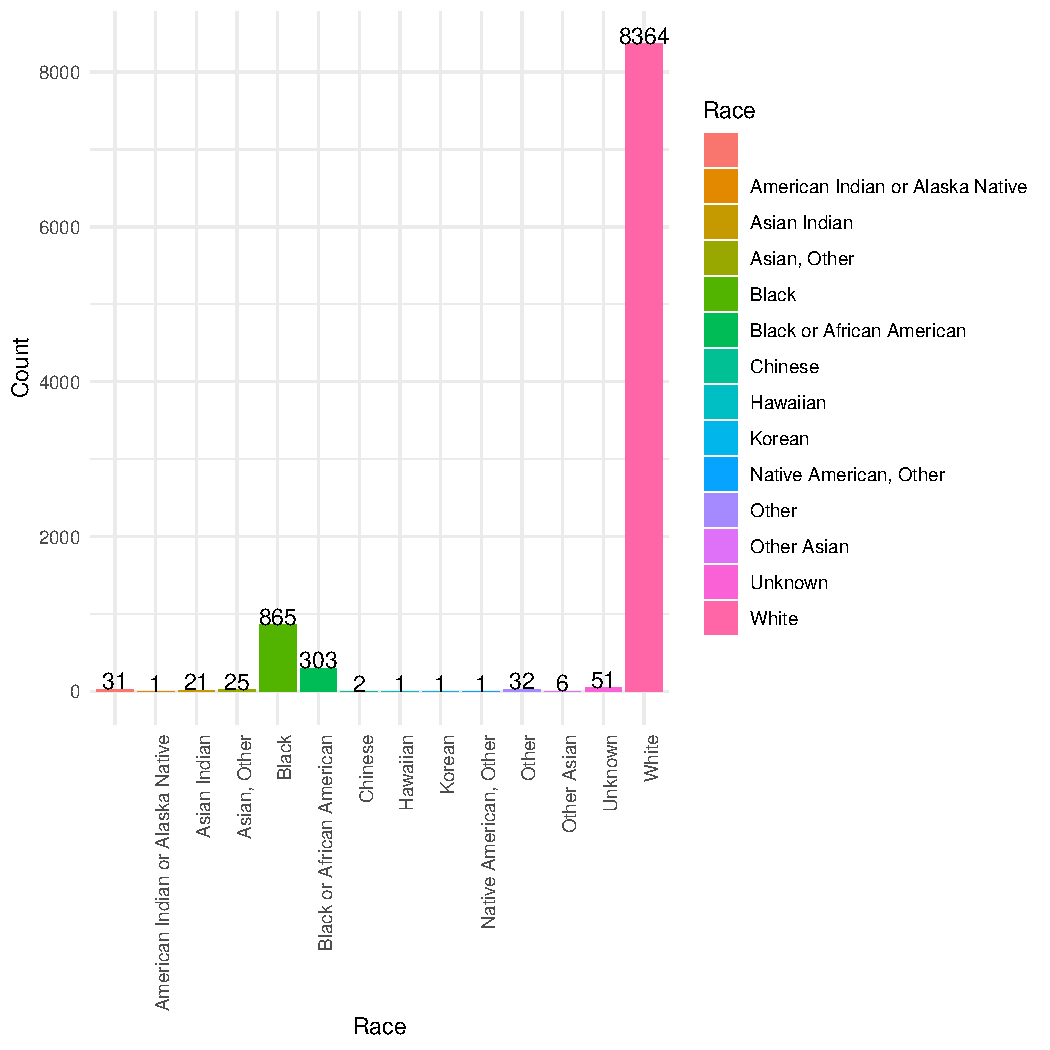
\includegraphics{RaceHist}
    \caption{Counts of drug overdoses by race.}
    \label{fig:RaceHist}
  \end{figure}

  \begin{figure}[tbp]
    \centering
    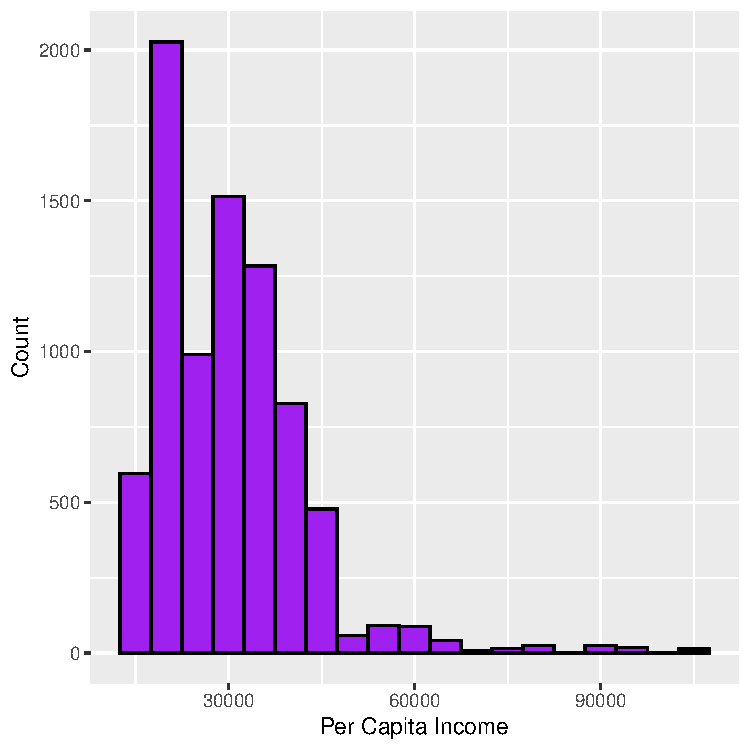
\includegraphics{AgeHistogram}
    \caption{Counts of Per Capita Income in the towns that the deceased lived in.  It is important to note that there were 1601 missing values.}
    \label{fig:MoneyHist}
  \end{figure}

The additional data that was created by adding the \citet{wikiwand_2023} to the drug overdose data was helpful in trying to determine the economic status of the deceased.  Per capita income is the mean income for every person in the city that the deceased lived in.  Histogram~\ref{fig:MoneyHist} shows that a majority of residents came from lower income communities, with the highest bar being represented as communities with a per capita income.  

\section{Discussion}\label{sec:Discussion}
Something that is important to note is that the demographics data from \citet{wikiwand2023} is from the 2010 census.  Although this is from outside the range of years in the study, this dataset was chosen due to the number of informative columns.  While the 2020 census data may have been better, this data should still do a good job of highlighting differences between towns.  While there may be minor changes between towns growing/shrinking and getting wealthier and poorer, the overall goal of being able to draw significance based on town was achieved.

It is very clear that the drug overdose epidemic is going to continue to plague Connecticut in the coming years.  While other states will be effected as well, this study is looking only at Connecticut.

One of the more interesting things about Graph~\ref{fig:Colorline} is how the number of overdose deaths tend to rise during the summer and fall during the winter.  A similar study that also looked at overdose deaths concluded that it was because of cultural factors in the United States and that longer days may be responsible for the increase in the summer \citep{han2022intentional}.  Additionally, the observance of many major religious and cultural holidays in the United States: Christmas, Hanukkah, and Kwanzaa may also play a role in reducing the number of overdose deaths during December.  \citet*{han2022intentional} also cited that suicide rates tend to come down during December, showing that the festive atmosphere that begins in December and lasts though New Year.  Thus, it is difficult to attribute the change in number of deaths to some measurable factor other than day length due to the confounding variables such as holidays and cultural atmosphere as presented above.

In terms of combatting the crisis, \citet{tran_2022} showed that there have been a substantial increase in opioid prescriptions from 1991 to 2013.  Opioid prescriptions rose from 76 million in 1991 to 207 million in 2013 with a peak of 219 million in 2011.  The drop-off in prescriptions in the last couple of years is likely the result of pharmacists and doctors beginning to combat the opioid crisis by trying to prescribe fewer opioids to their patients.  While it appears that there were some efforts to curb opioid prescriptions, the number of prescriptions in the last few years is so much more than what was prescribed in the 1990s.  In a practical sense 219 million opioid prescriptions is an exorbitant amount in a country of roughly 330 million, especially considering that opioids are generally not prescribed to minors.  

One of the more interesting graphs was Graph~\ref{fig:AgeHist}, which shows a bimodal distribution of ages.  It is the bimodal property of this graph that makes it intriguing.  This suggests that drug overdoses increase up until a certain point (35-36 years old), then decreases, then increases again (ages 49-50) before tapering off.  If we think about drug overdoses are related to drug use, then this suggests that it is middle-aged people (41-42) who have the lowest drug use amongst 27 to 61.  It is age range 25-27 that is the first age group to be higher than 41-42 and age range 59-61 that is the last.  The best explanation for this is that the distribution of ages in Connecticut is not uniform, and that the first hump represents drug use by young adults, which is to some degree expected, and the second hump is due to the Baby Boomer generation being larger than Generation X.  The timeline is a little difficult to understand due to the study occurring over a span of nine years, and further investigation is required to determine what was behind the bimodal age histogram.

Histogram~\ref{fig:RaceHist} shows that Whites are very well represented in drug overdose deaths, making up roughly 85\% of the graphic.  While this seems very high, it is important to keep in mind that 61.6\% of Connecticut is white according to the 2020 census \citep{acf2023}.  However, the \citet{data} does not contain the race ``Hispanic'' meaning that it may have been grouped in with ``white''.  As Hispanics make up 18.7\% of the Connecticut population, the total white and Hispanic population in Connecticut is 80.3\% which is very close to the 85\% found in overdose deaths.  The next largest minority in Connecticut are African Americans and Blacks, who are likewise represented in histogram~\ref{fig:RaceHist}.  It is clear that Asians are under-represented in the histogram, as they make up roughly 6\% of the Connecticut population but make up roughly 0.5\% of the drug overdoses in the data. Many of the other races included in the histogram do not constitute a large portion of the Connecticut population.  Histogram~\ref{fig:RaceHist} is not particularly informative as the results are about what is expected based on the demographics in Connecticut.

Poorer people were more likely to die of a drug overdose, as evidenced by Histogram~\ref{fig:EconHist}.  The highest bar in the histogram is for communities with a per capita income between \$5,000 and \$10,000.  For, reference in 2010 which is the same year the data is from, the per capita income in Connecticut was \$61,743 \citet{fred_2023}.  We are limited by not knowing the exact income of the deceased, but it is clear that it is the poorest people in Connecticut who are using drugs and making up drug overdose deaths.  There is a mark at \$60,000 on the graph and to the left of that graph there are a very limited number of deaths.  It is  important to note that there is a correlation between drug overdose deaths and per capita income, but it does not mean that having a low per capita income causes drug overdose death.  Drugs are often expensive and can effect one's ability to earn an income, meaning that the effect goes both ways: drugs can income and lower income may be indicative of a worse education and thus may increase the chances of somebody using and eventually dying of drugs.

One of the reasons that doctors may prescribe opioids and other medicines is because in some cases they are paid to.  A 2019 ProPublica study found that on average, doctors wrote 58\% more prescriptions if they were compensated by the drug company \citep{fresques_2019}.  For the drug Restasis, which is an eye medicine, doctors wrote 141\% more prescriptions if they received payment from the drugmakers.  Also concerning is that in 2016, one fifth of doctors who prescribed OxyContin, a very popular opioid, "had a promotional interaction with the drug's manufacturer, Purdue Pharma" \citep{fresques_2019}.  It is extremely problematic that companies are allowed to pay doctors to over-prescribe their medication, especially for addictive drugs such as OxyContin.  60 minutes has produced multiple reports on the Opioid crisis and how the Drug Enforcement Agency has not properly prosecuted or regulated the pharmaceutical industry due to lobbying and money \citep{cbs_2020}.  The opioid epidemic is not being resolved by the government due to the pharmaceutical industry's efforts to block the government agencies from doing their job, all while incentivizing doctors to peddle addictive drugs to their customers.  This is not something that is going to be easily resolved and is definitely not something that is going to go away anytime soon.  The trends in the data show that drug overdoses are rising, and I expect that to continue as it seems as if not enough is being done to combat this crisis.

\section{Appendix}
Here is the link to the data: \url{https://data.ct.gov/Health-and-Human-Services/Accidental-Drug-
Related-Deaths-2012-2021/rybz-nyjw}

\bibliographystyle{chicago}
\bibliography{references.bib}


\end{document}
